\documentclass{article}
\usepackage[utf8]{inputenc}
\usepackage{listings}
\usepackage{multicol}
\usepackage{amsmath}
\usepackage{color}
\usepackage{graphicx}
\usepackage[section]{placeins}


\usepackage{tikz}
\usepackage{algorithm, caption}
\usepackage[noend]{algpseudocode}
\usetikzlibrary{arrows}

\title{HyperLogLog: Analysis and implementation of an improved algorithm}
\author{Dequeker Chlo\'e, Ziat Ghiles}
\date{February 2015}

\begin{document}

\maketitle
\clearpage

\tableofcontents
\clearpage

\section{Introduction}
In this paper, we present our implementation and analysis of a
caridnality esmation algorithm proposed by Stefan Heule, Marc
Nunkesser and Alexander Hall: \texttt{HyperLogLog++}. This algorithm
is itself an improvement of the \texttt{HyperLogLog} algorithm
proposed by Flajolet et. al.

\subsection{cardinality estimation problem}
Finding the number of distinct elements in a data set with duplicates
is a well-known problem which applies in many fields.

The naive solution to this problem is to examine for each element of
the data stream its belonging to a data structure $\mathcal{D}$. If
$\mathcal{D}$ does not contain the element we add it to the data
structure. At the end of the process, the cardinality of the data
stream is equal to the size of $\mathcal{D}$.

This solution gives the exact answer but it is easy to see that it
scales very badly as the size of the data stream grows.

In order to resolve this problem, several alogorithms have been
proposed. These include LinearCounting and HyperLogLog which are the two
bases of the studied algorithm.

In this article we will first present the two algorithm cited above,
then we will detail our implementation, from the data structure used
to the differences we may have with the original article. Then we will
show the results of some benchmark we made in order to establish how
well the algorithm was functionning. In another section we will
explain how we made our implementation, and which language did we use.

\clearpage
\section{LinearCounting and HyperLogLog}
\subsection{Linear Counting}

Linear counting is an old algorithm originated from an article in
1990. The algorithm was at first mainly used in database application,
other application not being as used as now. This algorithm focuses on
using the number of empty indexes to determine an estimation of the
cardinality. The estimation can be stated as follows : $E = -m\times
log(V)$ where V is the proportion of empty indexes in our hashmap and
m is the size of the map (here with the precision indice $P=14$ we
have $m=2^{14}$).  We use this algorithm instead of the main one when
we try to estimate low values of cardinalities. One of the interest we
have in Linear counting is it's low bias even when we try to estimate
low cardinalities, and that is why we will use it under a certain
treshold.

\subsection{HyperLogLog}
The approach of the HyperLogLog algorithm to approximate the
cardinalities of a multiset is completely different. It is based on
randomization using a hash function for each element of the
multiset. It then focuses on the maximum of the number of leading
zeros in each hash values. it is legitimate to expect that the more
items there will be, the more this value will be high.  To improve the
precision of this calculation, HyperLogLog uses the stochastic
averaging technique: Doing so, it splits the stream in $m$ substreams,
and perform a computation separately on each.

At the end, a calculation that deduces from the expected value of the
number of leading zeros and the observed value of it the estimated
cardinality.\\
This result is then subjected to the following corrections:
\begin{itemize}
\item \emph{Small range correction :} As shown by simulation, for a
cardinality smaller than $\frac{5}{2}$ of the number of substreams, non-linear
distortions appear. For that range, LinearCounting is used.
\item \emph{Large range correction :} Due to the use of a 32 bit hash
function, when the cardinality goes to $2^{32}$, the chances of hash
collisions increases.
\end{itemize}

\section{HyperLogLog++}

\subsection{transition to 64 bits}
Using a 32-bits hash function restricts the area of efficiency of the
algorithm to the sets with less then $2^{32}$ distincts elements.
That's why an proposed improvement is to use a 64-bits hash function.
It does not significatively change the memory cost (it is
onlys increased only by 1 bit per substream).

\subsection{Bias estimation and correction}
For a given configuration of the algorithm, the observed bias is only
dependant on the cardinality estimated. From this observation, we
implement a correction method: As shown in figure 1, the raw
estimation of HLL is distorted for small cardinalities. In order to
correct this error, we take measures of it for cardinalities between 0
and 100 000 (with a step of 500) and we store them into a file. From
now, the file will be loaded at the begining of the calculation. A
correction may then be calculated for the result using a linear
interpolation between the values registered and the raw estimations.

\begin{center}
\begin{figure}[h]
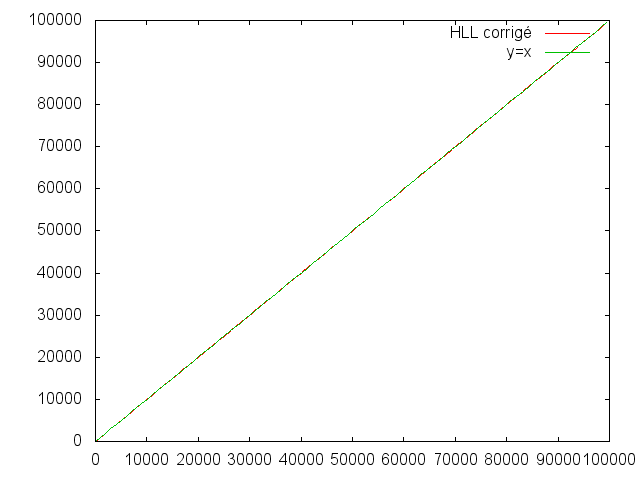
\includegraphics[scale=0.7]{img02.png}
\caption{Cardinality estimation for the corrected HLL}
\end{figure}
\end{center}


\subsection{Memory optimization}
Memory usage is an important factor in order to have a efficient
algorithm. In this algorithm, we can see that the size of the
different values we are using don't need to be of the standard size of
an int (which would be 4 bytes for a 32 bits integer). We need in fact
to keep two size of values, the first one being the index which
maximum value is $2^{P}$ with P the precision factor. That means any
index could be stocked on 14 bits. The second value is the number of
leading 0 of the hashed value which can't be over $64-P$ bits since we
work on a 64 bit version. The result is that the number of leading 0
will need 6 bits at most. The total size of those two values is then
of $6+P = 20$ bits. We will show in the next sections the different
kinds of compression we used during the implementation and in the
final state of the algorithm.

In this figure we observe the memory usage of the program. We can see
at first the map size increasing quickly, due to the fact that a lot
of indexes in the map are empty. As we will show below, the sparse
representation allows us to keep a small memory size. As soon as get
past the limit of the dense representation, we switch to it and
therefore keep a constant memory size, as well as a constant number of
bits used. Each time the size of the map in the sparse representation
becomes greater than the number of bits allocated, we double the size
of the allocated memory, resulting around the cardinality 12500 with a
peak of memory. Nevertheless we rapidly decrease the size of our
structure by switching to the dense mode (which is of constant
size).\\
 
 
\begin{center}
\begin{figure}[h]
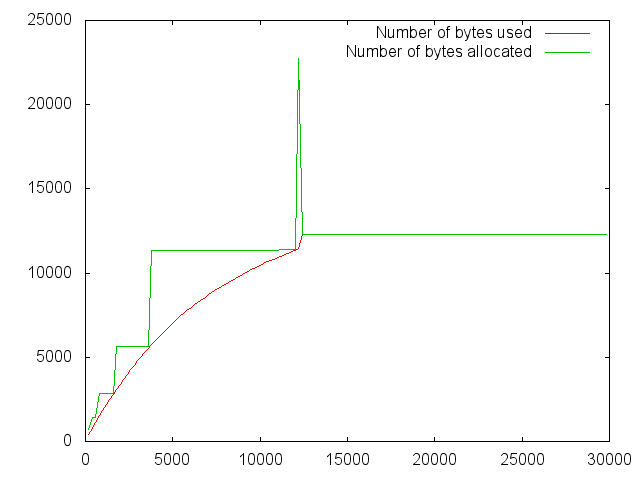
\includegraphics[scale=0.7]{plot_memoryUsage.png}
\caption{Cardinality estimation for the corrected HLL}
\end{figure}
\end{center}

\subsubsection{Sparse representation}
This is the first type of compression, and is the one which should be
used when only a low number of index have been hashed. This
representation works by pairs (index, number of leading zero (clz)).
For a better understanding consider a bitmap, then separate it by 20
bits blocks. Each of these block will be a pair (index, value). The
first P bits of the pair will represent the value of the index, and
the next 6 bits the value of clz. The total size (for P = 14) of the
bitmap will then be the number of different index hashed times 20
bits. We can then easily see why this representation is particularly
efficient for a low number of indexes and this is it's strong perk. On
the other hand, the more the number of different indexes grow, the
less efficient this representation becomes. \\ We will then introduce
the Dense representation, which becomes more efficient when the number
of indexes reaches certain value we will be talking about in the next
section. \\

\begin{center}
\begin{figure}[h]
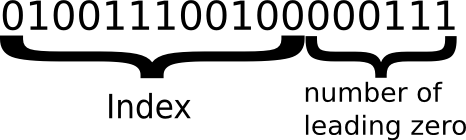
\includegraphics[scale=0.5]{sparse.png}
\caption{Sparse representation in a bitmap}
\end{figure}
\end{center}

This figure shows how is organized a sparse representation in the
bitmap we implemented.  The first 14 bits indicate the index's value,
and the 6 bits following represent the value of the number of leading
zero.

\subsubsection{Dense representation}
We will introduce in this section the second type of compression. As
we said earlier this representation if more efficient with a high
number of indexes. This picture this representation, we need here to
divid the bitmap by 6bits blocks. In this representation, when we go
through the first 6 bits of the bitmap, we will read the value of
index 0. The next 6 bits after that will be the value of index 1 and
so on. This representation allows us to represent the pair
(index,value) without writing the index. We can easily see this bitmap
will be of constant size since the value of the index is deducted from
the position of the 6-bit block in the bitmap. \\ Considering those
two representation, it is clear we need to start the algorithm using
the sparse representation, and then switch at some point to the dense
one. The limit where we want to switch from one to another is when the
sparse representation take more memory than the dense one. In the
implementation, it is then important to keep track of the bitmap's
size and switch to the dense representation whenever it is necessary.

\begin{center}
\begin{figure}[h]
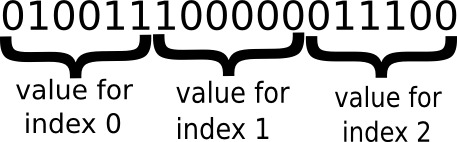
\includegraphics[scale=0.5]{dense.png}
\caption{Dense representation in a bitmap}
\end{figure}
\end{center}

In this figure, we can see that stocking the values for the first
three index takes only 18 bits, where it would take 60 in a sparse
representation.


\subsubsection{Varint encoding}
Since the temporary set used in the sparse representation is merged
with the list before it gets too large, performing a compression on it
is not as interesting then on the sorted list. We'll try to reduce the
memory usage of it by playing on two points:
\begin{itemize}
\item Using fixed-size integers as it is common practice in many
langages may here result in a waste of memory space.
\item Since the manipulated list is sorted, we can take advantage of
 this information.
 \end{itemize}

The \emph{variable length encoding} (also called varint encoding)
presents the perk of using a number of byte proportional to the value
it represents; It expoilts the fact that it is not necessary to use 32
bits if 8 are sufficient. That's why we use it to store the values
needed by the sparse representation.  We also use a \emph{difference
  encoding} besause of the good synergy it provides with the varint
encoding.  By storing differences between successives elements of the
list (Which is made possible by the fact that the list is sorted), the
stored values are smaller and require less memory space with the
varint encoding.

\begin{center}
\begin{figure}[!htb]
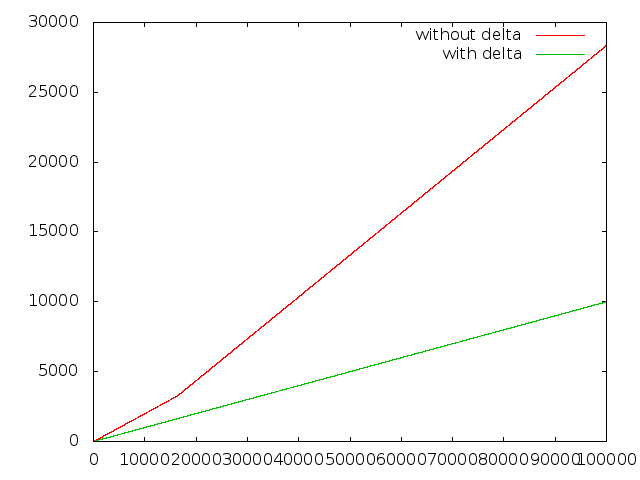
\includegraphics[scale=0.5]{img03.png}
\caption{Number of byte used with varint encoding (red) and both
  difference encoding and varint encoding (green)}
\end{figure}
\end{center}
\clearpage

\section{Conclusion}

In this section since this is mainly our personal point of view on the
work we've done. It appeared that we both had the same opinion about
this class:

 In conclusion, I though the class was great in general. Some point
 could be improved though. I find it weird that the two sub-part of
 the class are so divided, since we are still working on the same
 subject. My point is that the first part is almost only theoretical,
 and the second one is mainly oriented on the implementation of the
 algorithm.  I personally loved both (with maybe a preference for the
 second part), but I can easily understand that some people would be
 over bored with one part or another. It could then be great to mix
 the two parts. When we first introduced the basics notions of
 HyperLogLog, we could already have implemented the 32bits version for
 exemple.  On one hand there's the fact we need the theoretical
 knowledge to be able to understand what we actually are doing.  On
 the other hand, I could argue the implementation helps a lot with the
 understanding for the algorithm.

 Another note would be about how the work was presentated in the
 second part. During the pause we had in december and early january,
 we only had to implement the 32 bits version of the algorithm, which
 is in fact only the very begining of the whole project. The cause is
 that as we progress through the project during january, we were
 slowly overwhelmed with other projects. It could have been great to
 know the whole project as early as december, even if it meant to set
 the same objectives.

 In the organisation of the project, we managed to get along quite
 well, working on different parts of the project alone, and some other
 parts were done with the two of us (mainly when it meant to implement
 functions of each other).
 \end{document}
